\chapter{Low level control}\label{chap:llc}




REWREITE!!!
The low level control is all implemented on a Digilent Nexys 2 test kit, featuring a spartan 3 fpga from Xilinx.
Architecturally, it is split in two nearly independent systems, one being the SPI driver and the other being the motor control.
They communicate through a shared RAM (uddyb type) block, but functions otherwise completely independant of each other.


\section{Motor interface}
The motor interface is responsible for presenting an easy to use interface to the arm processor, making it possible to control the motor torque and receive feedback in the form of pan and tilt position and velocity.
All communication is done through the RAM block as seen on figure \ref{fig:FPGAMotorArchitecture}, which means that the interface functions independently of the SPI implementation.

\subsection{Overall architecture}
The motor interface is split into two distinct parts. The PWM controller, which generates a pwm signal from a given input and a decoder controller, which reads the decoder pins, and tracks position and velocity.

A top level module is introduced to handle all memory interfacing. It houses all the individual component instances, and binds them together.

The output pins of the PWM controller A and B, is connected to the three pins of each H-bridge.
The input pins of the decoder system comes from the index pins of the hall sensors mounted on the pan/tilt system and the decoder A and B signal from the two output pins on the motors.

\begin{figure}[htb]

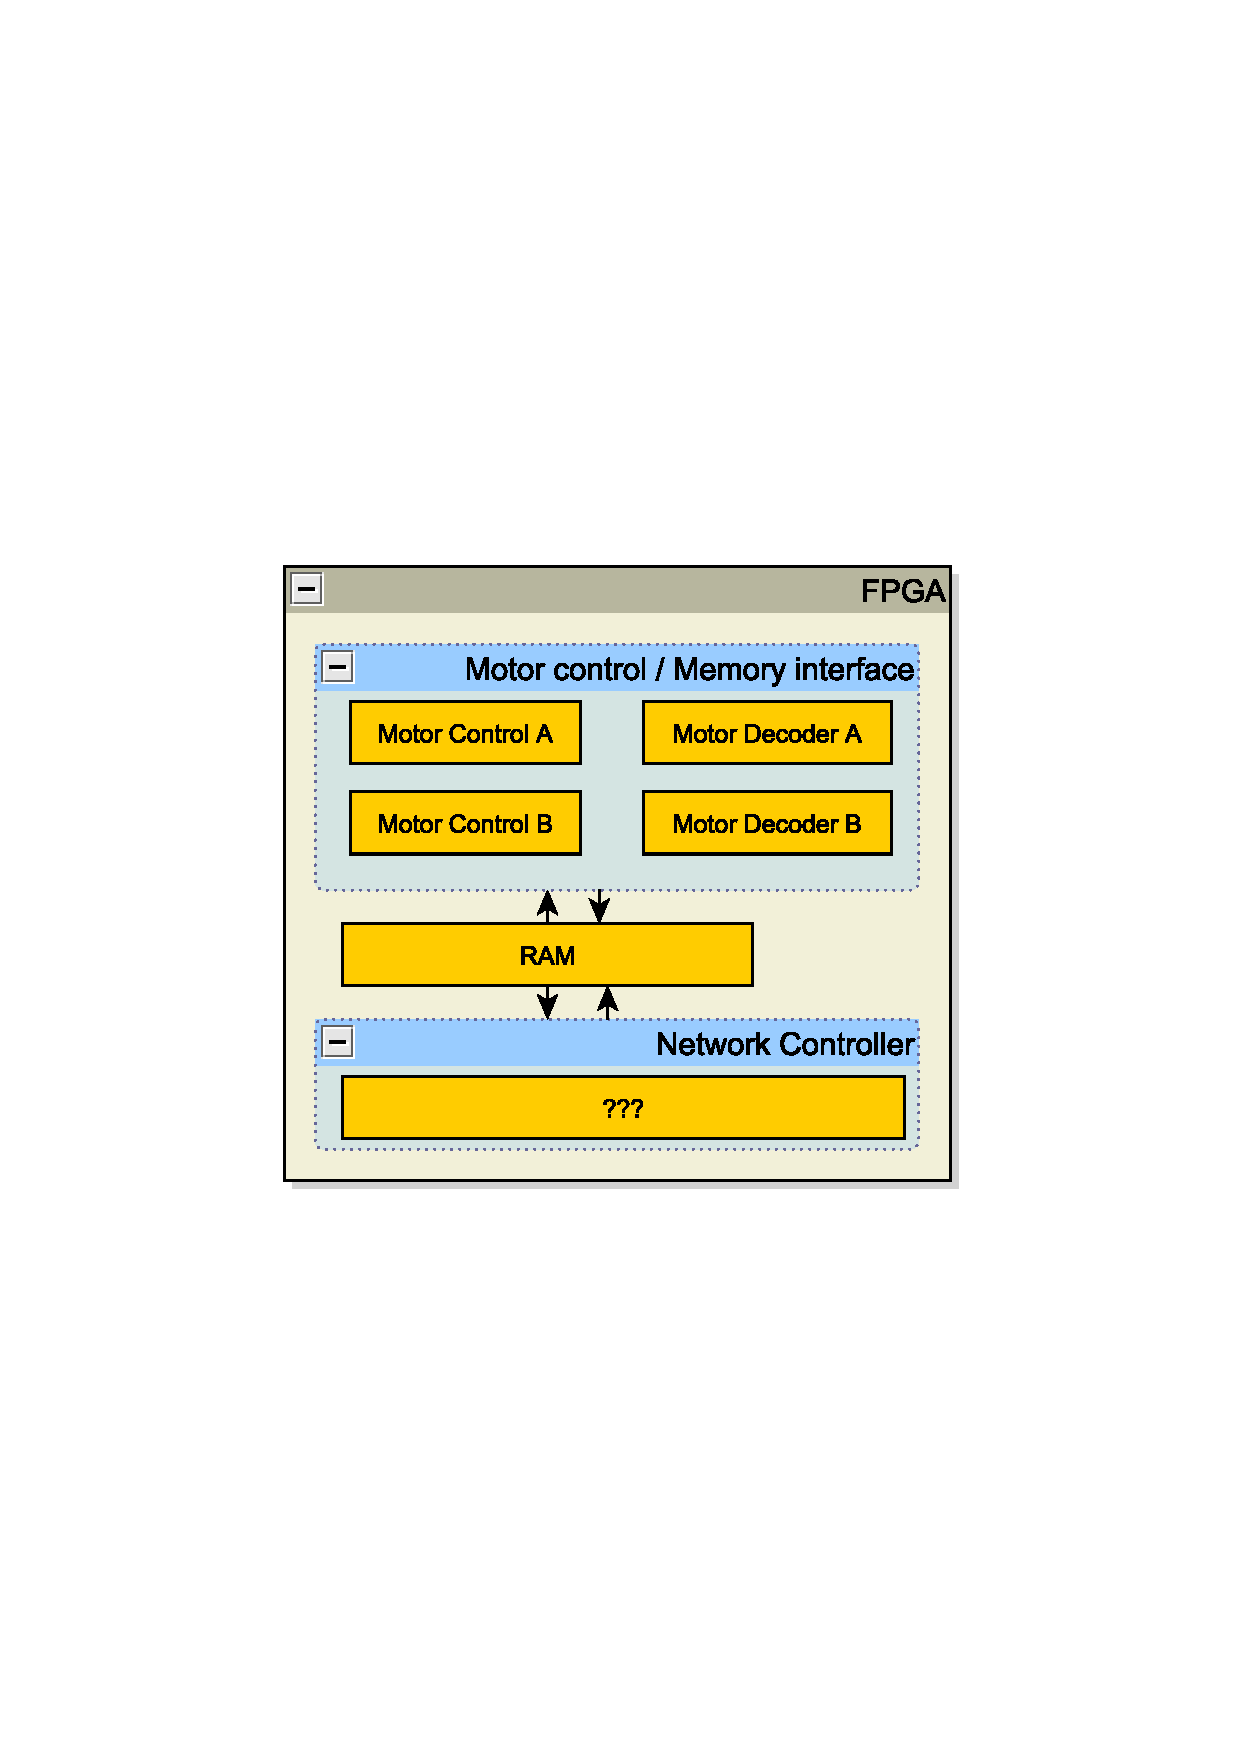
\includegraphics[scale=0.6,clip,trim=135 270 135 270]{FPGAmotorarchitecture.pdf}

\caption{FPGA architecture, from the motor interface perspective}
\label{fig:FPGAMotorArchitecture}
\end{figure}

\subsection{Memory layout}
The memory layout is as seen on table \ref{tab:Memorymapping}. The position is represented by an unsigned bit, centered around 0x8000, this is because it is easier to calculate the position without considering a sign, and it would make no difference for the control system on the arm whether the position is represented by signed or unsigned numbers.
Velocity as output and duty cycle as input is represented as a 16 bit signed twos-complement value.
This is because the sign bit makes it easy to read what the desired motor direction is.
The aux register reads position reset, and motor freerun command bits. It also sets two bits, representing whether the hall sensors indicate that the system is in zero position.



\begin{table}[htb]
\centering
\begin{tabular}{|l|r|}
\hline
Address & Value \\
\hline
0x02 & DUTY A MSB \\
0x03 & DUTY A LSB\\
0x04 & DUTY B MSB\\
0x05 & DUTY B LSB\\
0x06 & POS A MSB\\
0x07 & POS A LSB\\
0x08 & POS B MSB\\
0x09 & POS B LSB\\
0x0a & VEL A MSB\\
0x0b & VEL A LSB\\
0x0c & VEL A MSB\\
0x0d & VEL A LSB\\
0x0e & AUX FROM ARM\\
0x0f & AUX TO ARM\\
\hline 
\end{tabular}
\caption{Memory locations of control registers}
\label{tab:Memorymapping}
\end{table}


\section{Motor control block}


The motor control block is split into 3 seperate modules.
The PWM generator, the signed-to-magnitude splitter, and the Motor AUX control as seen on figure \ref{fig:pwmblock}.
It takes a 16 bit signed integer and a control bit as input, indicating whether the motor should be driven by a pwm signal, or if it should be set in free run mode. 
When the motor is not in free run, the enable pin on the H-bridge is high, and the pwm signal changes between the braking and running state. If the free run bit is set, the H-bridge is disabled and no pwm signal is generated.

\begin{figure}[htb]
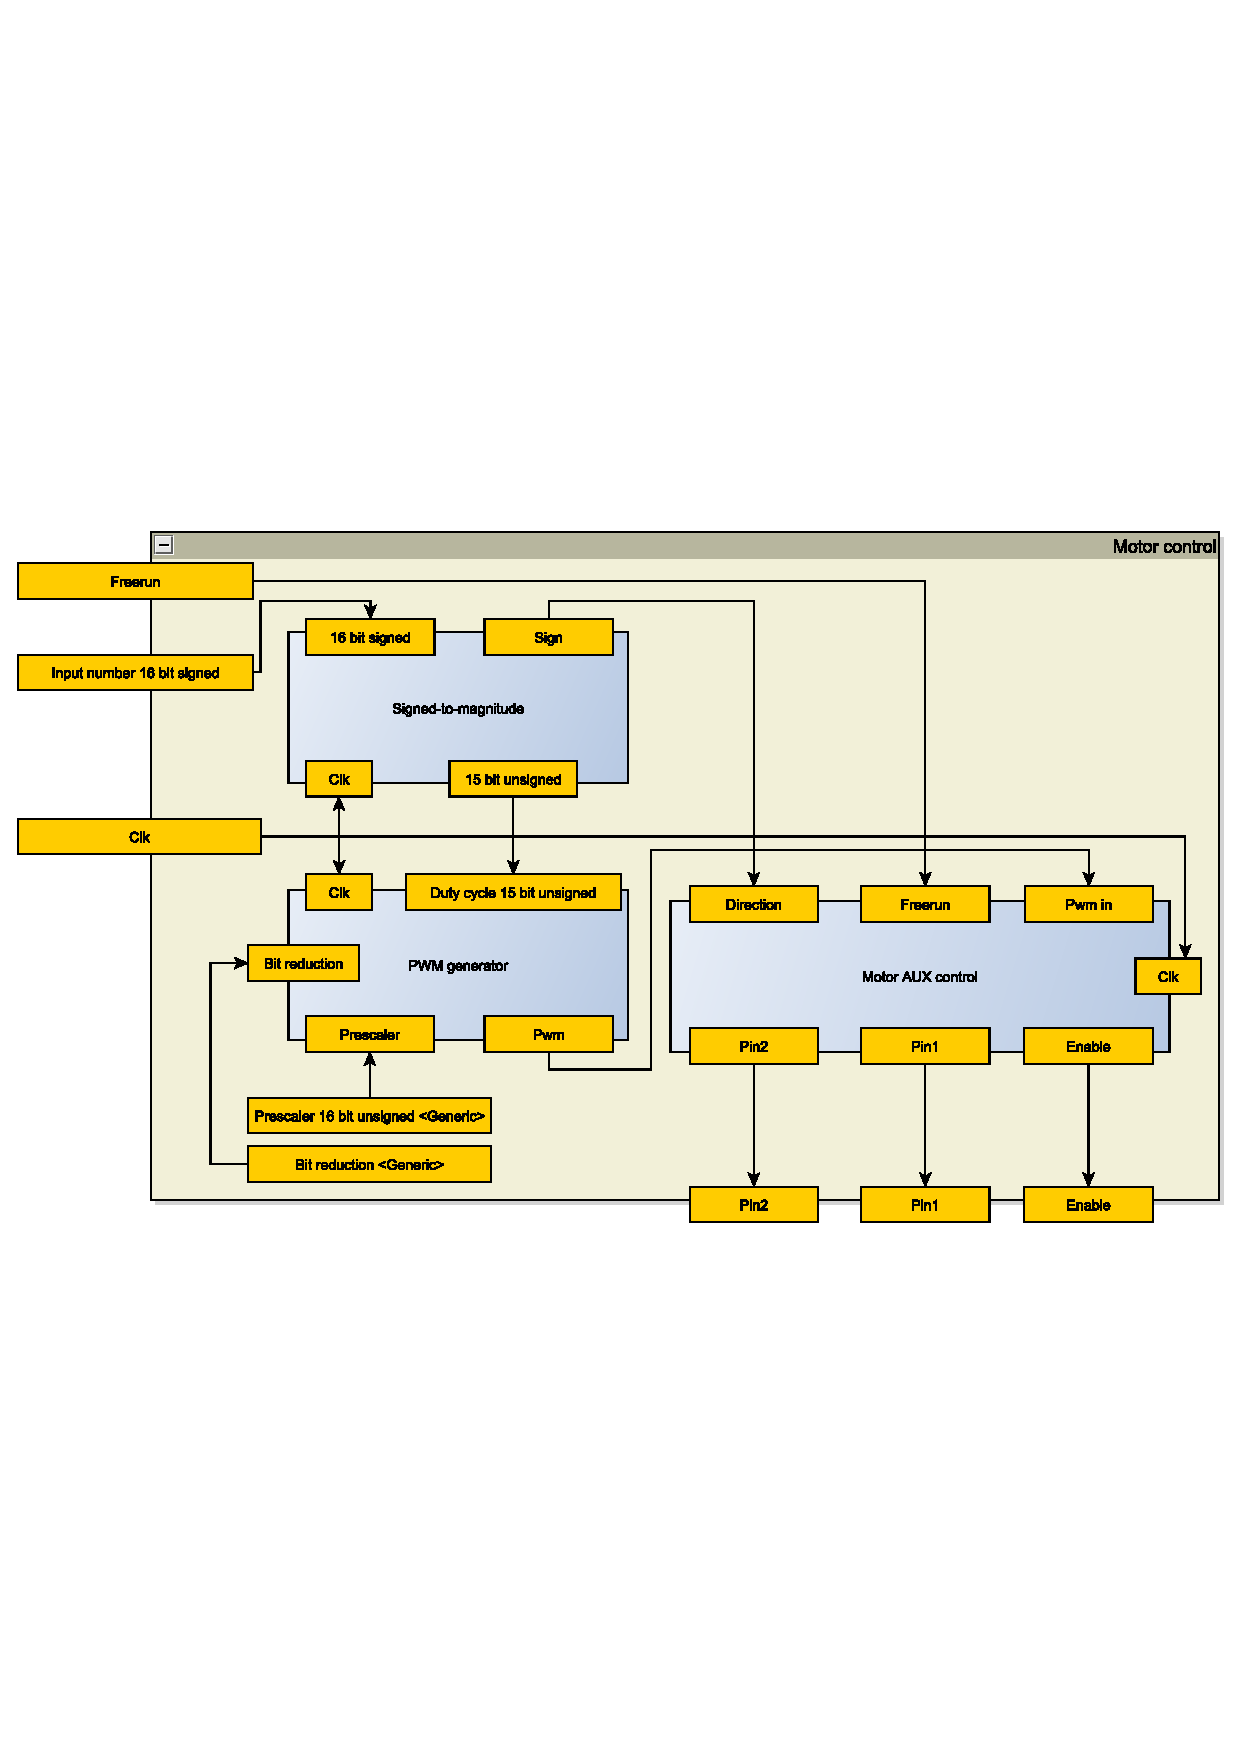
\includegraphics[scale=0.6,clip,trim=0 250 10 250]{PWMblock.pdf}
\caption{Block/signal layout of the Motor control block}
\label{fig:pwmblock}
\end{figure}

\subsection{PWM generator}
The PWM generator takes a clk signal and a duty cycle (15 bit unsigned value) as input. It also takes two generic parameters as input. A prescaler value to decrease the frequency, and a bit reduction parameter to increase it. These allows the PWM block to be configured for a desired frequency.

Internally the pwm generator consists of a counter register that is decremented each tick as seen of figure \ref{fig:pwmchart}. If the counter is less than the input, the output is 1 otherwise it is zero.
If the counter value underflows, it is set to the second highest value it can represent. This ensure that the PWM block is able to output high and low value dc if needed, at the cost of lacking an extra bit of resolution.

The bit reduction parameter effectively reduces the amount of significant bits in the counter and value signals.
The prescaler is used to introduce a delay between each tick.

The frequency of the PWM needs to be at around 20khz or above. If it is lower than that it is in the audible range of frequencies which would be an annoyance. If the frequency is too high, to much energy is lost in the transistors, not to mention the fact that an h-bridge has a switching time, which would distort the actual duty cycle output.

For calculating the pwm frequency the following formula is used: 
\begin{equation}
F_{pwm} = \frac{F_{xtal}}{2^{number of bits}}
\end{equation}

Without using prescaler and bit reduction values, the pwm frequency is calculated with 16 bit resolution and a 50 mhz internal clock, which gives a resulting frequency:
\begin{equation}
\frac{50 mhz}{2^{15}} = 1525.88 hz
\end{equation}

This is way to low, and therefore the amount of used bits are reduced by four giving the frequency:
\begin{equation}
\frac{50 mhz}{2^{11}} = 24414.1 hz
\end{equation}
Which is just above the minimum frequency requirement.

\begin{figure}[htb]
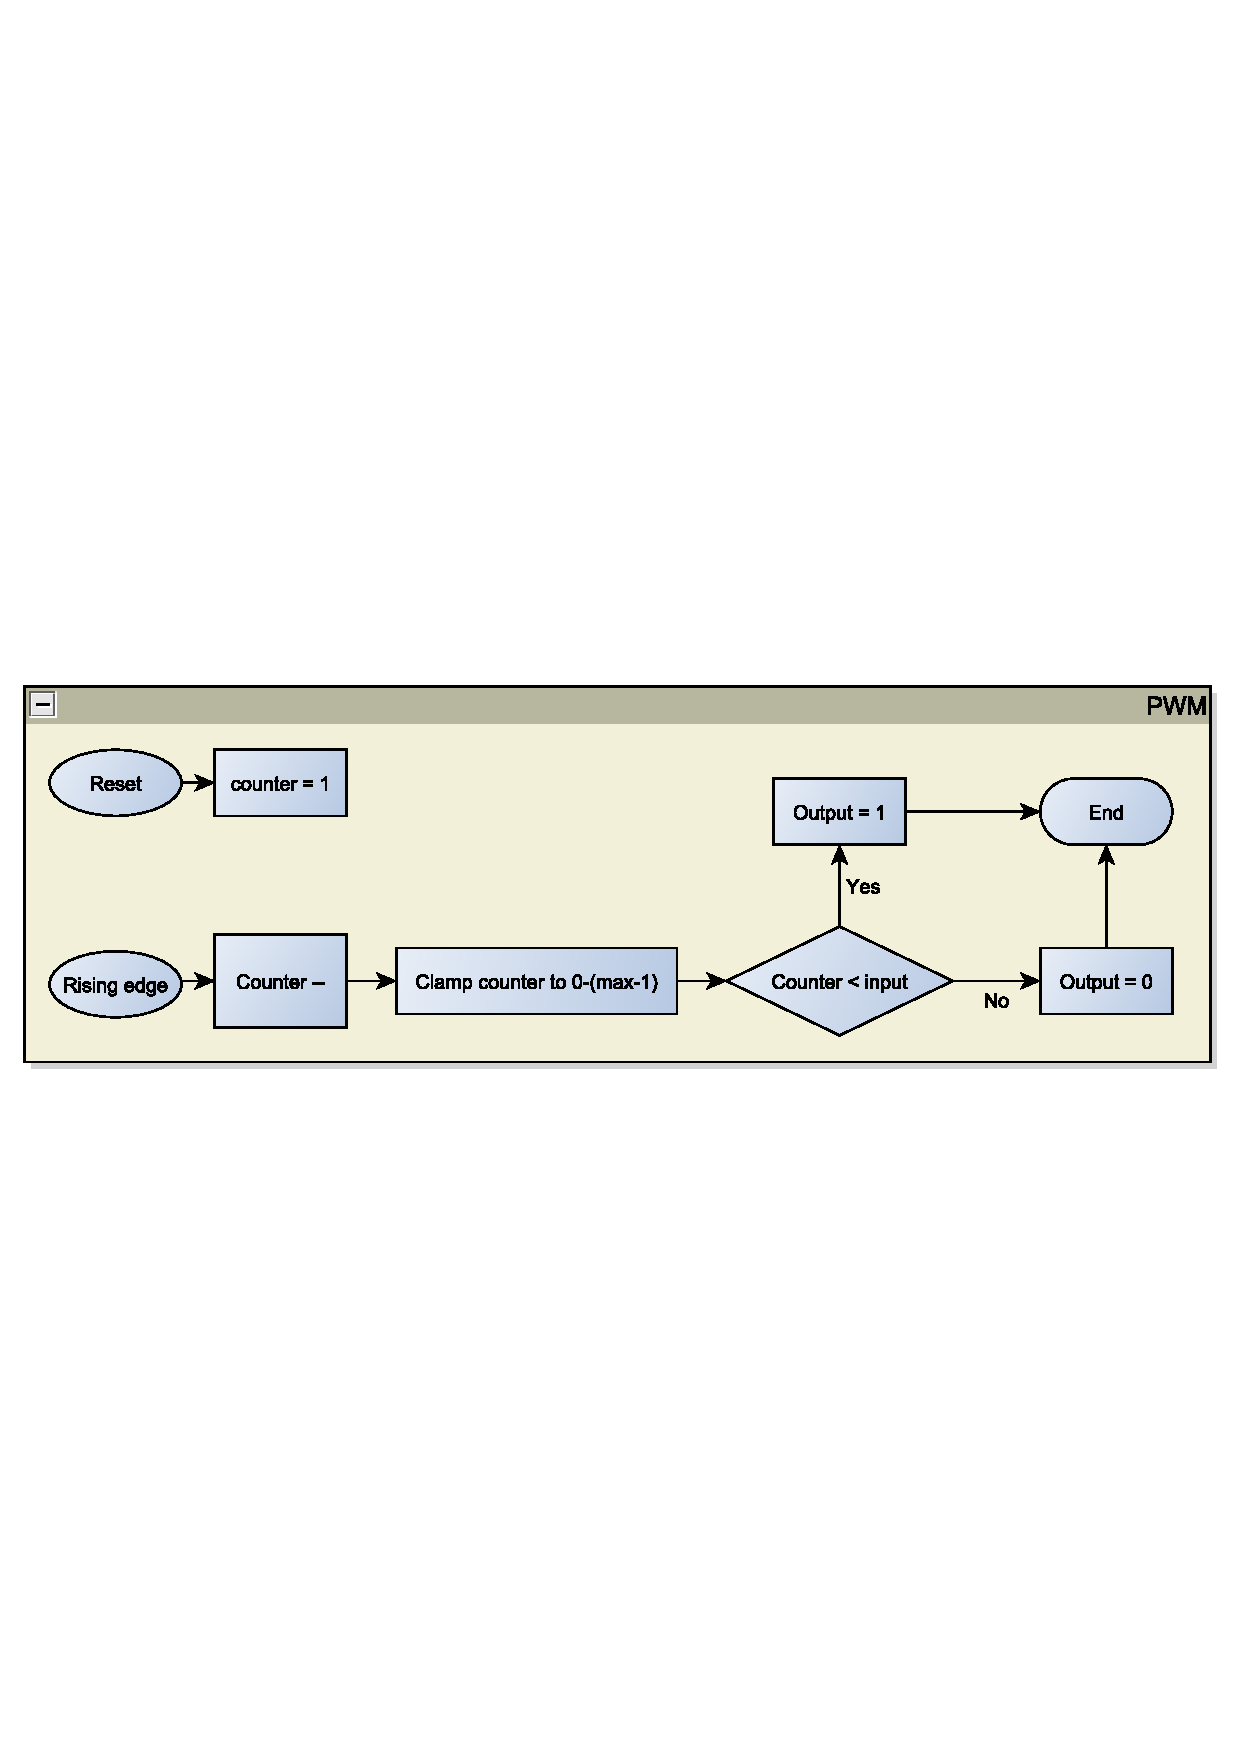
\includegraphics[scale=0.6,clip,trim=10 330 10 330]{PWMexecution.pdf}
\caption{Flowchart of the pwm generator}
\label{fig:pwmchart}
\end{figure}

\subsection{Signed-to-magnitude splitter}
The signed-to-magnitude splitter takes a signed 16 bit integer as input and outputs the sign and magnitude separately.
The magnitude is computed as follows:
If it positive, its just the 15 last bits, if it is negative the twos compliment value is the output.

\subsection{AUX control}
The aux control takes the direction, pwm and freerun signals as input, and output the pwm signal on either pin 1 or 2 of the h-bridge. If the freerun pin is not high, the enable pin is high, if the freerun pin is high, no pwm is output, and the enable pin is low.

\section{Decoder system}
The decoder system is responsible for reading the state of the pan/tilt system from the hall sensors mounted on the system, and the quadrature encoders on the motors. 
It outputs a relative position from the reset point and a velocity for each of the two axes, as precise as possible.

The decoder is split into 4 major components: The Input filtering, the quadrature decoder, position normalizer and velocity estimator components, as seen on figure \ref{fig:decoderblock}. 



\begin{figure}[htb]
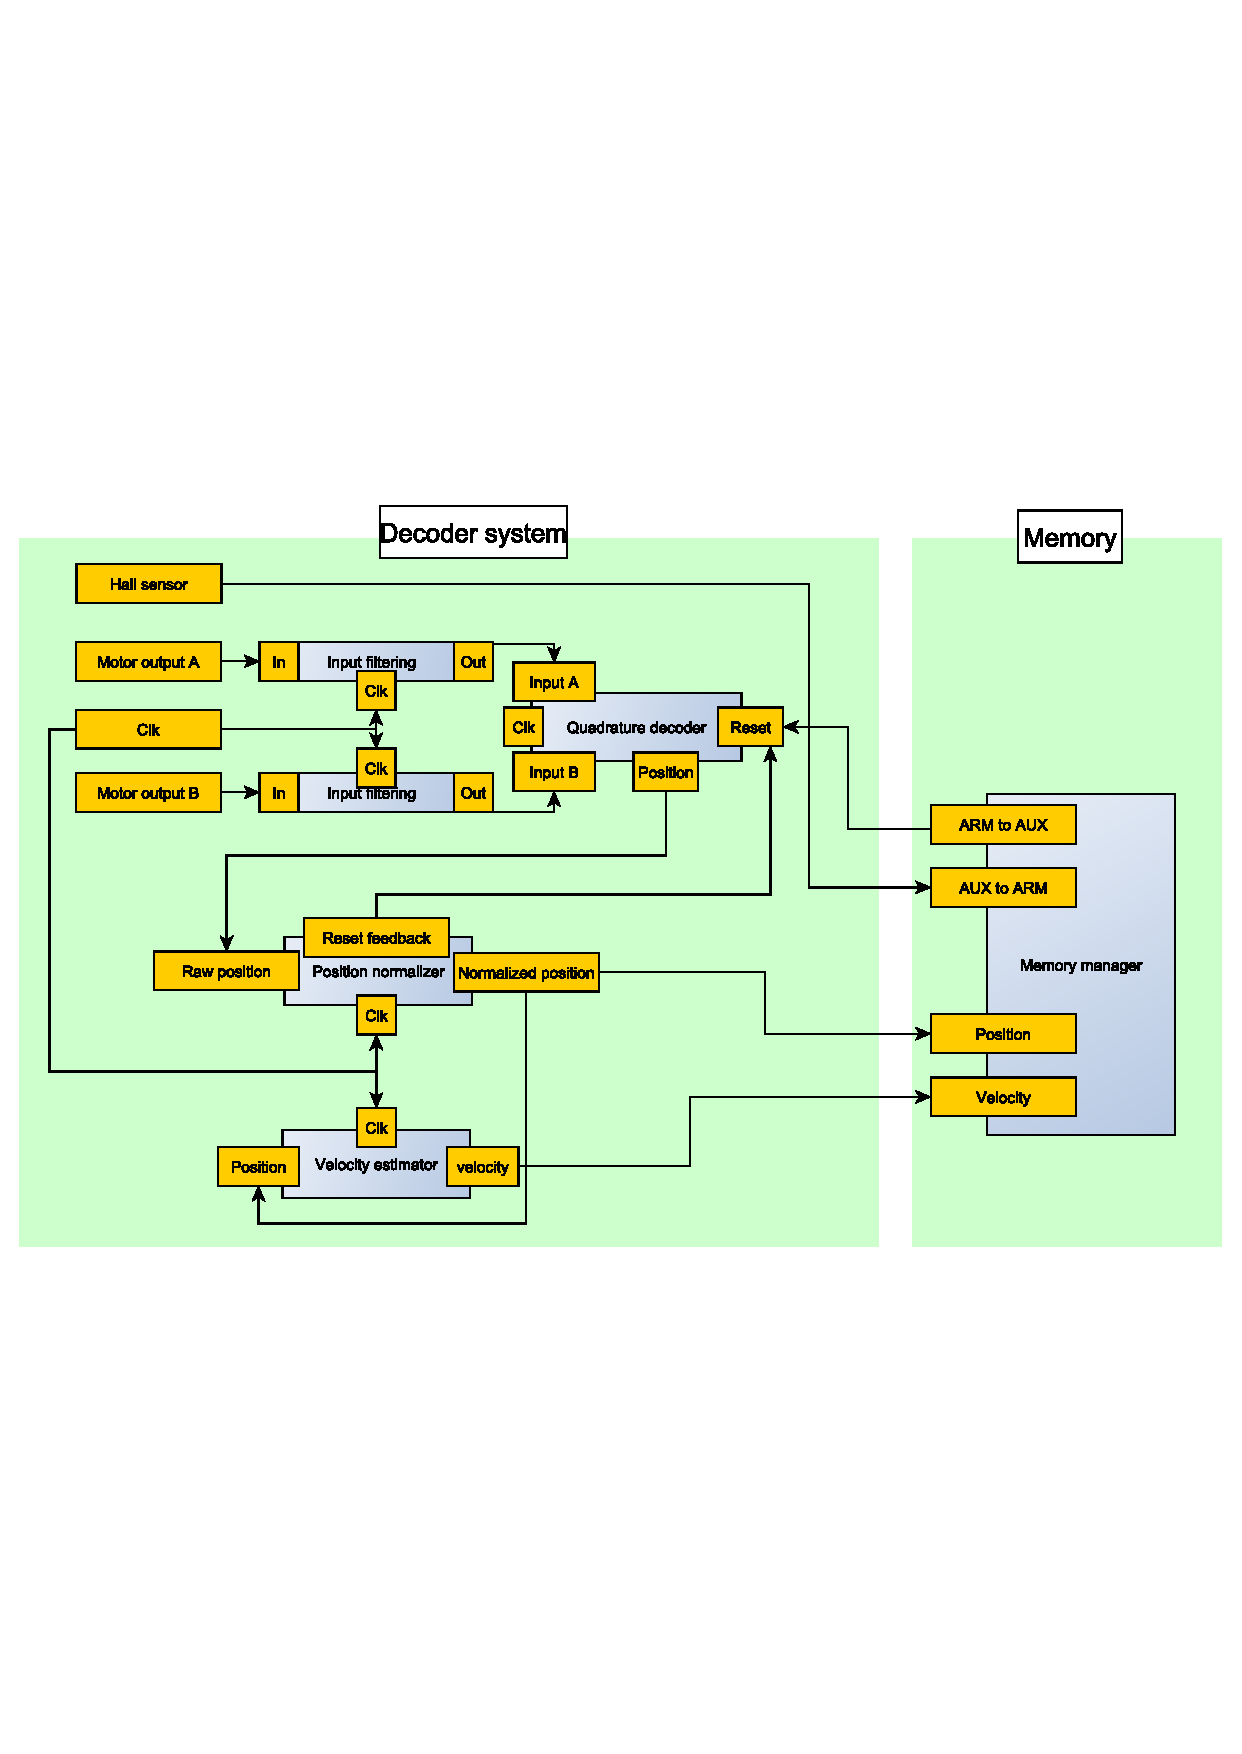
\includegraphics[scale=0.6,clip,trim=2 250 2 230]{decoderblock.pdf}
\caption{Block/signal layout of the decoder system}
\label{fig:decoderblock}
\end{figure}


\subsection{Input filtering}
Since the input signal comes from the outside \"real\" world, unwanted noise must be removed for it to be used. However, the regulator depends on this signal, so care must be taken not to introduce an unwanted large delay, as that would make the signal  useless.

To remove noise, a simple de-bounce, with hysteresis is applied, it features a counter that, for every clock pulse counts up if the input signal is high and down if it is low.
When ever the counter rises above a threshold, and the filter is outputting a low signal, it changes to high. The same opposite when counting down.
The counter part of the process introduces a delay in output changes, so that a lot of switching back and forth between high and low, will not affect the output. The hysteresis helps negate short burst errors in the input. 

The distance between the lowest value possible in the hysteresis counter, and the value that causes a switch to high the in output,

The difference between the hysteresis counters lowest value and the rising edge value, or the highest value and the falling edge value, whichever is highest, determines the maximum frequency the input filter will let through, as well as the delay introduced in the position counter.

A set of values must be chosen that filters the signal adequately, without producing error signals. The tilt rotor has been observed to have approximately 1000 ticks pr. full revolution, and with full power to the motors, max one rotation pr. second.
This means that the input filter should be able to let a 1khz signal through at least. \\ 
Since external forces can temporarily push the system to higher frequencies, it is assumed that a max frequency of 1mHz should cover all but the most extreme cases.

This means that the maximum input delay can be 50 clock ticks.
In this assignment, a set of values was then chosen within the constraints: 
Lowest value: 0
Maximum value: 20
Low hysteresis: 4
High hysteresis: 16

These values give a maximum input delay of 16 clock ticks(320 ns) which is sufficient for this application.

\subsection{Quadrature encoder}
The quadrature encoders job is to convert the two decoded signals from the motor, to a relative position. The signal is generated from two hall sensors that are positioned 90 degrees apart. Giving 4 different output states, each state indicating what quadrant the motor is positioned in, an example of the signal can be seen in figure \ref{fig:decodersignal}.
\begin{figure}[htb]
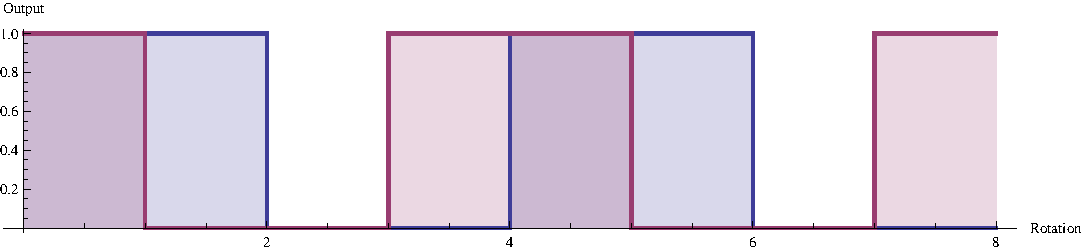
\includegraphics[scale=0.6,clip,trim=0 0 0 0]{ddecodersignal.pdf}
\caption{Example decoder output from a motor with constant speed}
\label{fig:decodersignal}
\end{figure}
The decoding process can be thought of as a state machine (with the encoder output being the state variable), where a state transition corresponds to a movement step in one of two directions.
When the decoder is first powered, a default position value is kept, and then incremented or decremented according to the statetransition. The default value is set at 0x8000 unsigned integer, as this allows for the maximal displacement in either direction. 
Overflow is not handled in this module, as it is not its job to know anything about the configuration the motor is in, however an external reset pin is provided, which returns the counter to 0x8000. (This reset signal is incidentally powered by the position normalizer module).
The situation where the input pins both change in one clock cycle is not handled by the system.

\begin{figure}[htb]
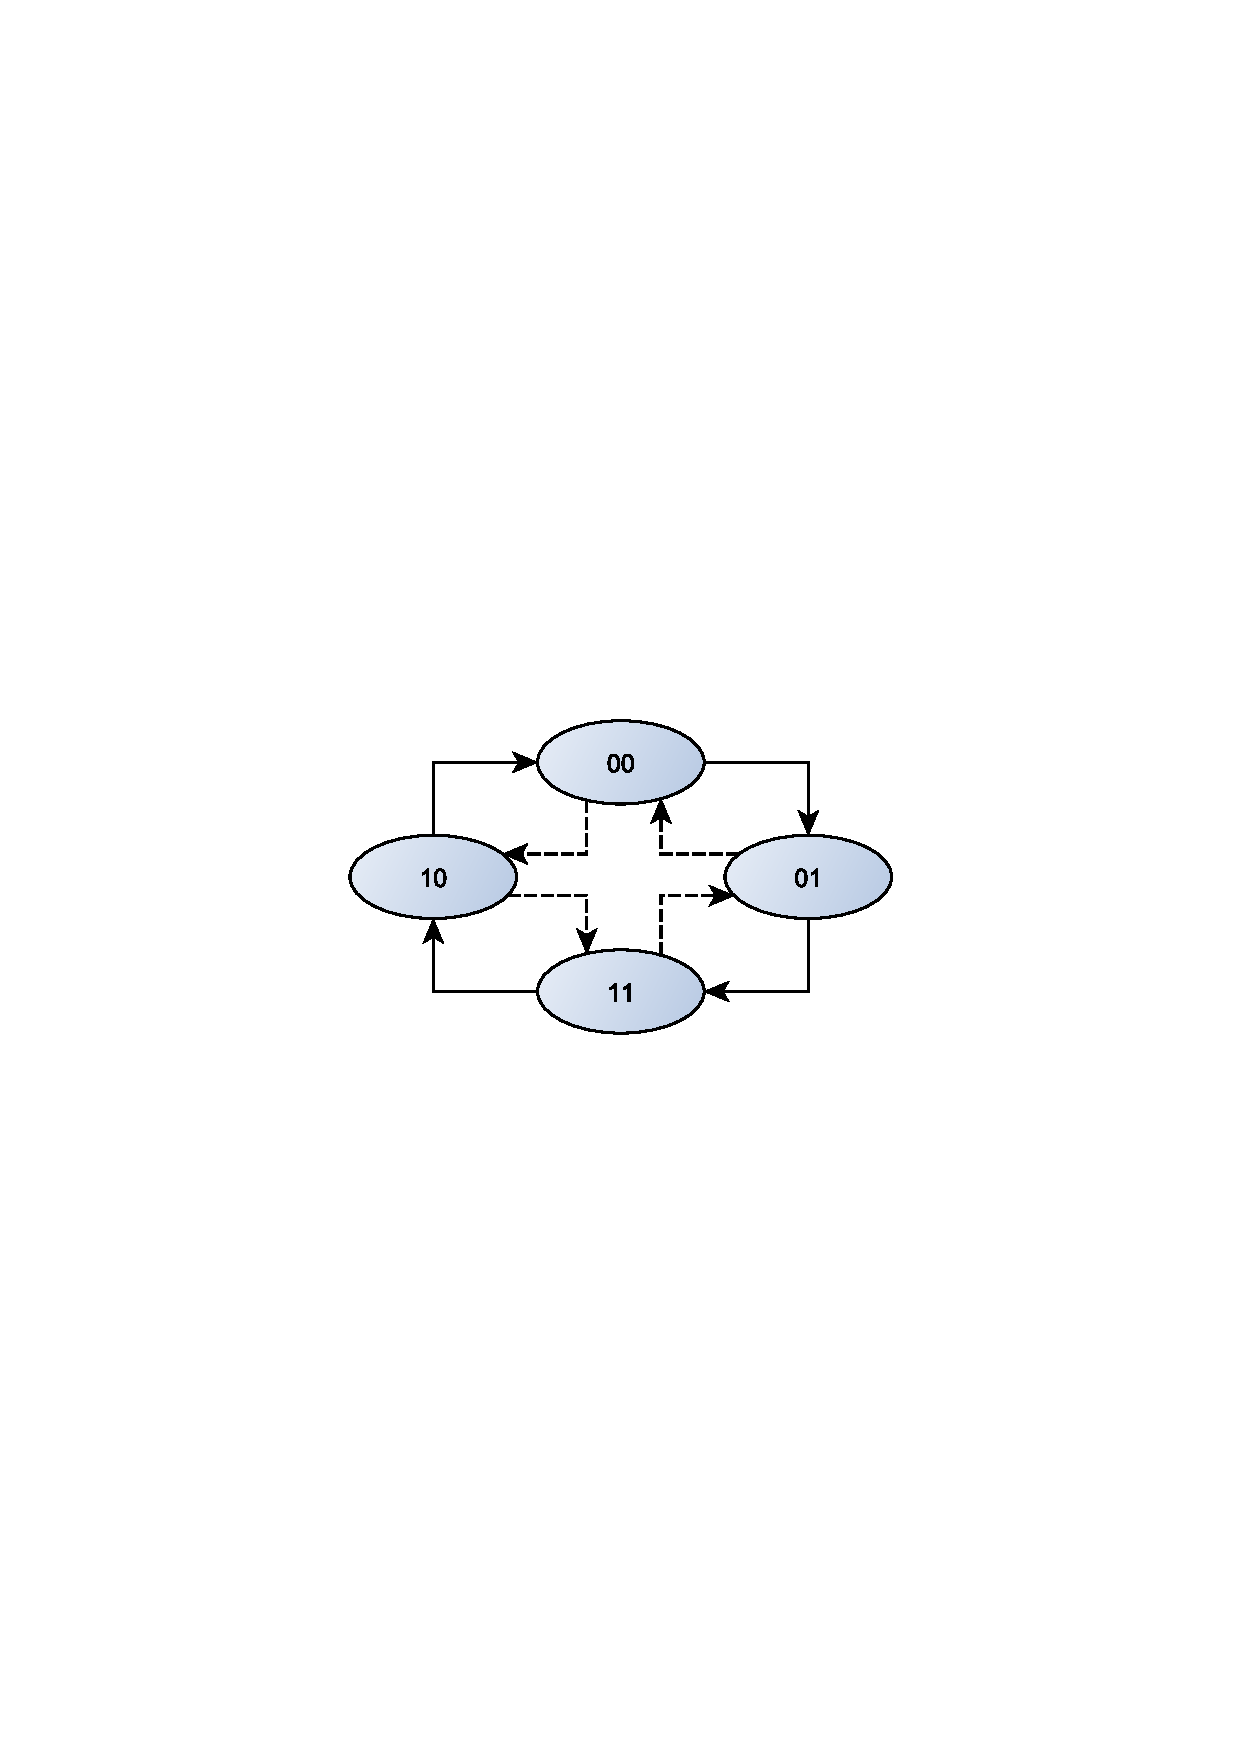
\includegraphics[scale=0.6,clip,trim=130 330 130 330]{decoderstates.pdf}
\caption{State diagram of the decoder module, the stipled arrows indicate a negative clockwise, the solid indicate a counter-clockwise or vice verca.}
\label{fig:decoderstate}
\end{figure}

\subsection{Position normalizer}
The position normalizer block is used for any conversions/adaptations of the raw position value necessary. For instance the position could be converted to radians or similar. It also features a feedback reset signal, if this should be necessary. 
In the final version of the application, this block does nothing other than let the input go directly to the output.
Should any automatic reset system be required, based on the position, this is the block to handle it.

\subsection{Velocity estimator}
The velocity estimator is responsible for measuring the velocity based on the counter input.
There are several methods available for measuring the velocity, each with its drawbacks and strengths.
A simple method is to compare the position with a fixed frequency, so that for instance each second, the velocity is the difference between the position before and after a second has passed. This has the advantage of being easy to implement and test, also everything is implemented with integers. The drawback is that this method can produce wildly varying velocity measurements, especially if the actual velocity produces a position change frequency just above or below the sampling frequency.
This drawback can be offset by \"tuning\" the sampling frequency until a desirable behavior has been reached.
Another method is the secant method, where the time between each change of the position is measured. The reciprocal of this is then the velocity. The advantage of this method is that it is, in theory, very precise. The drawback is that a floating/fixed point division is necessary, in order to obtain the correct result. Also should there be any imprecision in the motor decoding, it will be reflected strongly in the measured velocity. Furthermore, a time-out period must be included, for there is no edge to detect when the motors stop moving.

In both cases smoothing of the result can be needed. By using a running average filter, the velocity measurement can be smoothed over many samples, but a first order delay in the measurement is introduced.

In the final application, there is no velocity estimator, since it is not needed in the chosen regulation method, however the two mentioned measurement methods are included in the codebase for completeness sake.


\section{Watchdog}
Since all control commands are buffered in the ram until updated again, the fpga has no way of knowing if the SPI link has been lost, either because of the ARM processor crashing, or cable failure etc. This means that in case the case of the link being lost, it will continue going if any velocity command has been issued before the connection died. To correct this problem, a watchdog is implemented. It outputs an enable signal as long as there is a link between the fpga and ARM. 
To detect the link presence, two registers in the control register are constantly incremented, and the watchdog keeps a watch on them, should they fail to change within a set time, the watchdog will stop all motor activity.
The watchdog module is not included in the final application due to time constraints.
